\documentclass[12pt]{article}

\usepackage[utf8]{inputenc}
\usepackage[T1]{fontenc}
\usepackage[english]{babel}
\usepackage[a4paper, margin=2.3cm]{geometry}
\usepackage{amsmath, amssymb}
\usepackage{bm}
\usepackage{parskip}
\usepackage{graphicx}
\usepackage{float}
\usepackage{caption}
\usepackage{subcaption}
\usepackage{booktabs}
\usepackage{xcolor}
\usepackage{csquotes}
\usepackage[backend=biber, style=numeric, backref=true]{biblatex}
\usepackage{xurl}
\usepackage[colorlinks=true, linkcolor=blue, citecolor=blue, urlcolor=blue]{hyperref}

\addbibresource{../references.bib}
\graphicspath{{../figures/}}
\newcommand{\nRaw}{53{,}488}
\newcommand{\rawStart}{01 January 2016 00:00}
\newcommand{\rawEnd}{06 February 2022 17:00}
\newcommand{\nMissingHours}{2}
\newcommand{\missingHours}{30 October 2016 01:00 and 31 October 2021 01:00}
\newcommand{\priceMatch}{100.0}
\newcommand{\consRatioMin}{2.000}
\newcommand{\consRatioMax}{2.000}
\newcommand{\corConsBuy}{0.972}
\newcommand{\meanCons}{4{,}141}
\newcommand{\meanBuy}{4{,}088}
\newcommand{\meanNpCons}{8{,}282}
\newcommand{\nKnots}{318}
\newcommand{\knotWeekday}{Friday}
\newcommand{\nAfterLastKnot}{63}
\newcommand{\nNoReservoir}{71}
\newcommand{\nMissingPrice}{2{,}562}
\newcommand{\nMissingPriceAll}{2{,}562}
\newcommand{\missPriceTopYear}{2018}
\newcommand{\missPriceTopN}{858}
\newcommand{\missPriceRuns}{1{,}509}
\newcommand{\missPriceMaxRun}{13}
\newcommand{\missPriceRunsShort}{82}
\newcommand{\nClean}{50{,}855}
\newcommand{\pctRemoved}{4.9}
\newcommand{\cleanStart}{04 January 2016}
\newcommand{\cleanEnd}{06 February 2022}
\newcommand{\nNeg}{10}
\newcommand{\nZero}{1}
\newcommand{\nNonPos}{11}
\newcommand{\minPrice}{\ensuremath{-}1.97}
\newcommand{\maxPrice}{600.16}
\newcommand{\maxPriceTime}{21 December 2021 at 17:00}
\newcommand{\nAboveTwoHundred}{246}
\newcommand{\nAboveTwoHundredPct}{0.5}
\newcommand{\nYearTwentyTwo}{883}
\newcommand{\meanPrice}{39.0}
\newcommand{\medianPrice}{32.4}
\newcommand{\sdPrice}{32.5}
\newcommand{\meanConsClean}{4{,}143}
\newcommand{\sdCons}{1{,}344}
\newcommand{\minConsClean}{1{,}636}
\newcommand{\maxConsClean}{8{,}133}
\newcommand{\minRes}{7.1}
\newcommand{\maxRes}{99.8}
\newcommand{\meanPriceYI}{26.5}
\newcommand{\meanPriceYII}{29.2}
\newcommand{\meanPriceYIII}{44.1}
\newcommand{\meanPriceYIV}{39.3}
\newcommand{\meanPriceYV}{9.1}
\newcommand{\meanPriceYVI}{74.9}
\newcommand{\meanPriceYVII}{138.8}
\newcommand{\meanResYI}{60.2}
\newcommand{\meanResYII}{58.4}
\newcommand{\meanResYIII}{59.7}
\newcommand{\meanResYIV}{63.3}
\newcommand{\meanResYV}{68.9}
\newcommand{\meanResYVI}{59.6}
\newcommand{\meanResYVII}{43.5}
\newcommand{\hourMinMean}{34.2}
\newcommand{\hourMinAt}{3}
\newcommand{\hourMaxMean}{43.2}
\newcommand{\hourMaxAt}{8}
\newcommand{\monthMinMean}{28.3}
\newcommand{\monthMinAt}{June}
\newcommand{\monthMaxMean}{59.5}
\newcommand{\monthMaxAt}{December}
\newcommand{\corPriceCons}{0.21}
\newcommand{\corPriceRes}{\ensuremath{-}0.02}
\newcommand{\corConsRes}{\ensuremath{-}0.31}
\newcommand{\corYearRes}{0.03}
\newcommand{\corYearCons}{0.00}
\newcommand{\corYearPrice}{0.37}
\newcommand{\nScatterSample}{10{,}000}
\newcommand{\nAboveYlim}{109}
\newcommand{\nPar}{49}
\newcommand{\rTwo}{0.667}
\newcommand{\rTwoPct}{66.7}
\newcommand{\rse}{18.75}
\newcommand{\dfRes}{50{,}806}
\newcommand{\nullDev}{53.71}
\newcommand{\resDev}{17.87}
\newcommand{\aicFull}{442{,}519}
\newcommand{\bicFull}{442{,}961}
\newcommand{\bIntercept}{52.27}
\newcommand{\seIntercept}{1.27}
\newcommand{\ciLIntercept}{49.78}
\newcommand{\ciUIntercept}{54.77}
\newcommand{\bHourNight}{\ensuremath{-}2.04}
\newcommand{\seHourNight}{0.59}
\newcommand{\ciLHourNight}{\ensuremath{-}3.19}
\newcommand{\ciUHourNight}{\ensuremath{-}0.88}
\newcommand{\bHourMorning}{5.25}
\newcommand{\seHourMorning}{0.59}
\newcommand{\ciLHourMorning}{4.09}
\newcommand{\ciUHourMorning}{6.42}
\newcommand{\bHourEvening}{4.37}
\newcommand{\seHourEvening}{0.59}
\newcommand{\ciLHourEvening}{3.21}
\newcommand{\ciUHourEvening}{5.53}
\newcommand{\bApr}{\ensuremath{-}31.99}
\newcommand{\seApr}{0.69}
\newcommand{\ciLApr}{\ensuremath{-}33.35}
\newcommand{\ciUApr}{\ensuremath{-}30.64}
\newcommand{\bJul}{18.65}
\newcommand{\seJul}{0.75}
\newcommand{\ciLJul}{17.17}
\newcommand{\ciUJul}{20.12}
\newcommand{\bDec}{33.41}
\newcommand{\seDec}{0.45}
\newcommand{\ciLDec}{32.53}
\newcommand{\ciUDec}{34.28}
\newcommand{\bSat}{\ensuremath{-}3.03}
\newcommand{\seSat}{0.32}
\newcommand{\ciLSat}{\ensuremath{-}3.65}
\newcommand{\ciUSat}{\ensuremath{-}2.41}
\newcommand{\bSun}{\ensuremath{-}4.20}
\newcommand{\seSun}{0.32}
\newcommand{\ciLSun}{\ensuremath{-}4.83}
\newcommand{\ciUSun}{\ensuremath{-}3.57}
\newcommand{\bYeighteen}{18.11}
\newcommand{\seYeighteen}{0.29}
\newcommand{\ciLYeighteen}{17.53}
\newcommand{\ciUYeighteen}{18.69}
\newcommand{\bYtwenty}{\ensuremath{-}9.87}
\newcommand{\seYtwenty}{0.31}
\newcommand{\ciLYtwenty}{\ensuremath{-}10.47}
\newcommand{\ciUYtwenty}{\ensuremath{-}9.27}
\newcommand{\bYtwentyone}{48.97}
\newcommand{\seYtwentyone}{0.29}
\newcommand{\ciLYtwentyone}{48.41}
\newcommand{\ciUYtwentyone}{49.54}
\newcommand{\bYtwentytwo}{108.94}
\newcommand{\seYtwentytwo}{0.72}
\newcommand{\ciLYtwentytwo}{107.53}
\newcommand{\ciUYtwentytwo}{110.35}
\newcommand{\bCons}{2.08}
\newcommand{\seCons}{0.17}
\newcommand{\ciLCons}{1.74}
\newcommand{\ciUCons}{2.42}
\newcommand{\bRes}{\ensuremath{-}0.71}
\newcommand{\seRes}{0.011}
\newcommand{\ciLRes}{\ensuremath{-}0.73}
\newcommand{\ciURes}{\ensuremath{-}0.69}
\newcommand{\hNight}{03}
\newcommand{\hMorning}{08}
\newcommand{\hEvening}{17}
\newcommand{\bResTen}{\ensuremath{-}7.1}
\newcommand{\bResTenAbs}{7.1}
\newcommand{\ciLResTen}{\ensuremath{-}7.3}
\newcommand{\ciUResTen}{\ensuremath{-}6.9}
\newcommand{\bConsOne}{2.1}
\newcommand{\bConsSD}{2.8}
\newcommand{\bResSD}{\ensuremath{-}18.8}
\newcommand{\bResSDAbs}{18.8}
\newcommand{\sdConsGWh}{1.34}
\newcommand{\sdResPct}{26.4}
\newcommand{\peakDiff}{7.3}
\newcommand{\wdayPMax}{0.580}
\newcommand{\nHourNotSig}{5}
\newcommand{\dRtwoHour}{0.27}
\newcommand{\dRtwoMonth}{7.25}
\newcommand{\dRtwoWeekday}{0.20}
\newcommand{\dRtwoYear}{44.19}
\newcommand{\dRtwoConsumption}{0.10}
\newcommand{\dRtwoReservoir}{2.86}
\newcommand{\dAICHour}{370}
\newcommand{\dAICMonth}{10{,}003}
\newcommand{\dAICWeekday}{295}
\newcommand{\dAICYear}{42{,}966}
\newcommand{\dAICConsumption}{144}
\newcommand{\dAICReservoir}{4{,}192}
\newcommand{\FHour}{18.1}
\newcommand{\FMonth}{1{,}006.4}
\newcommand{\FWeekday}{51.3}
\newcommand{\FYear}{11{,}247.2}
\newcommand{\FConsumption}{145.6}
\newcommand{\FReservoir}{4{,}367.6}
\newcommand{\minF}{18.1}
\newcommand{\rTwoCal}{0.637}
\newcommand{\rTwoCalPct}{63.7}
\newcommand{\rTwoYearOnly}{55.9}
\newcommand{\vifHour}{1.7}
\newcommand{\vifMonth}{79.8}
\newcommand{\vifWeekday}{1.1}
\newcommand{\vifYear}{1.5}
\newcommand{\vifConsumption}{7.8}
\newcommand{\vifReservoir}{11.7}
\newcommand{\vifadjHour}{1.01}
\newcommand{\vifadjMonth}{1.22}
\newcommand{\vifadjWeekday}{1.01}
\newcommand{\vifadjYear}{1.03}
\newcommand{\vifadjConsumption}{2.79}
\newcommand{\vifadjReservoir}{3.42}
\newcommand{\auxResMonth}{89.4}
\newcommand{\auxResYear}{2.6}
\newcommand{\auxResAll}{91.4}
\newcommand{\auxConsMonth}{76.4}
\newcommand{\auxConsYear}{1.6}
\newcommand{\auxConsAll}{87.1}
\newcommand{\pctOutThree}{1.08}
\newcommand{\pctOutThreeNormal}{0.27}
\newcommand{\nOutThree}{551}
\newcommand{\maxResid}{489.1}
\newcommand{\skewResid}{6.09}
\newcommand{\kurtResid}{94.6}
\newcommand{\resSDYI}{10.7}
\newcommand{\resSDYII}{8.7}
\newcommand{\resSDYIII}{11.6}
\newcommand{\resSDYIV}{12.3}
\newcommand{\resSDYV}{9.1}
\newcommand{\resSDYVI}{38.3}
\newcommand{\resSDYVII}{25.5}
\newcommand{\pctLagOneIsHour}{97.0}
\newcommand{\acfOne}{0.961}
\newcommand{\acfTwentyfour}{0.743}
\newcommand{\acfWeek}{0.509}
\newcommand{\pacfOne}{0.961}
\newcommand{\pacfTwo}{\ensuremath{-}0.191}
\newcommand{\pacfTwentyfour}{\ensuremath{-}0.044}
\newcommand{\dw}{0.078}
\newcommand{\dwP}{\ensuremath{<0.001}}
\newcommand{\dwRho}{0.961}
\newcommand{\hacRatioMin}{2.2}
\newcommand{\hacRatioMax}{15.3}
\newcommand{\seHacCons}{1.50}
\newcommand{\pHacCons}{0.164}
\newcommand{\ciLHacCons}{\ensuremath{-}0.85}
\newcommand{\ciUHacCons}{5.01}
\newcommand{\seHacRes}{0.152}
\newcommand{\pHacRes}{\ensuremath{<0.001}}
\newcommand{\ciLHacResTen}{\ensuremath{-}10.1}
\newcommand{\ciUHacResTen}{\ensuremath{-}4.1}
\newcommand{\seHacMorning}{1.35}
\newcommand{\pHacMorning}{\ensuremath{<0.001}}
\newcommand{\seHacJul}{6.76}
\newcommand{\seHacYtwentyone}{4.38}
\newcommand{\pHacSun}{\ensuremath{<0.001}}
\newcommand{\binResMax}{10.2}
\newcommand{\binResMin}{\ensuremath{-}4.7}
\newcommand{\binConsMax}{2.4}
\newcommand{\binConsMin}{\ensuremath{-}1.8}
\newcommand{\kIndexCons}{1.00}
\newcommand{\kIndexRes}{0.44}
\newcommand{\binTopLo}{47}
\newcommand{\binTopHi}{60}
\newcommand{\binTopPctDec}{9}
\newcommand{\binTopResWithDec}{10.2}
\newcommand{\binTopResNoDec}{2.5}
\newcommand{\edfCons}{8.9}
\newcommand{\edfRes}{8.9}
\newcommand{\gamDevDiff}{1.75}
\newcommand{\gamF}{343.2}
\newcommand{\gamFp}{\ensuremath{<0.001}}
\newcommand{\gamDf}{16.1}
\newcommand{\rTwoGam}{0.700}
\newcommand{\rTwoGamPct}{70.0}
\newcommand{\rseGam}{17.81}
\newcommand{\aicGam}{437{,}297}
\newcommand{\bicGam}{437{,}880}
\newcommand{\dAICGam}{5{,}222}
\newcommand{\dBICGam}{5{,}081}
\newcommand{\kMax}{9}
\newcommand{\gamResBumpAt}{53}
\newcommand{\gamResTenToForty}{21.9}
\newcommand{\gamResBumpToNinetyFive}{58.1}
\newcommand{\gamResFortyToBump}{7.1}
\newcommand{\gamConsTwoToSeven}{1.7}
\newcommand{\gamConsSevenToEight}{42.9}
\newcommand{\nConsAboveSeven}{992}
\newcommand{\pctConsAboveSeven}{2.0}
\newcommand{\pctConsAboveSevenCrisis}{1}
\newcommand{\meanPriceConsAboveSeven}{62.0}
\newcommand{\nCrisis}{3{,}811}
\newcommand{\meanPriceCrisis}{125.5}
\newcommand{\meanResCrisis}{66.2}
\newcommand{\resDecTwentyOne}{71.0}
\newcommand{\resvDecTwentyOne}{60.8}
\newcommand{\priceDecTwentyOne}{174.3}
\newcommand{\pctOutThreeCrisis}{80}
\newcommand{\edfGamTotal}{64.8}
\newcommand{\aicCal}{446{,}897}
\newcommand{\bicCal}{447{,}321}


\newcommand{\bs}[1]{\boldsymbol{#1}}
\newcommand{\eur}{EUR/MWh}

\title{STAT201 Project: What drives the hourly electricity price in NO1?\\[0.3em]
\large A Gaussian GLM with calendar effects, consumption and reservoir level}
\author{Sondre Erdi Solbakken}
\date{October 2026}

\begin{document}

\maketitle

\begin{abstract}
\noindent
I model the hourly day-ahead electricity price in the Norwegian bidding zone NO1 ($n = \nClean$ hours, 2016 to early 2022) with a Gaussian GLM with identity link. The predictors are hour, month, weekday and year as factors, plus consumption and the weekly reservoir fill level. The model explains $R^2 = \rTwo$ of the variation. The year factor accounts for most of this, then month and reservoir level, while consumption adds almost nothing beyond the calendar factors. Ten percentage points more water in the reservoirs is linked with a price about \bResTenAbs{} \eur{} lower. The residuals are strongly autocorrelated, so the usual standard errors are far too small. With autocorrelation-robust standard errors the reservoir effect remains clear, but the consumption effect does not. A GAM shows non-linear effects and improves AIC by \dAICGam, but the main picture stays the same.
\end{abstract}

%------------------------------------------------------------
\section{Introduction}

In my master thesis I work with data from the Nordic power market, and for this project I use part of that data (approved by my professor instead of a Kaggle data set). The topic is the day-ahead electricity price in NO1, the bidding zone around Oslo and the south-east of Norway. Every day Nord Pool sets one price for each hour of the next day. NO1 has a lot of consumption, so I expect the price to follow demand with a daily and a seasonal pattern. At the same time most Norwegian power comes from hydro, so the amount of water stored in the reservoirs should matter.

The response variable is the hourly day-ahead price in \eur. The research question is:

\begin{displayquote}
How much of the variation in the hourly NO1 price can be explained by the time of day, the season, the weekday, the year, the consumption and the reservoir fill level, and which of these matter most?
\end{displayquote}

My working hypothesis was that demand matters and that the reservoir level matters even more. I report what the data shows, also where it does not agree. All calculations are done in R \parencite{R} with the script \texttt{R/project.R}, and every number in this report comes from that script.

%------------------------------------------------------------
\section{Data and preparation}\label{sec:data}

\subsection{Source and variables}

The data comes from the data set I built for my master thesis (\texttt{dataset\_timeseries.csv}), with one row per hour from \rawStart{} to \rawEnd{} UTC ($\nRaw$ rows) and columns for several Nordic zones. I use three NO1 columns: the day-ahead price from Nord Pool \parencite{nordpool} in EUR per MWh, the consumption in MWh for the hour, and the reservoir filling degree from NVE \parencite{nve}, which I use in percent. I also used the raw Nord Pool download (\texttt{nordpool\_2016-01-01\_2022-11-30.h5}) to check the price and consumption. Both files are read in R with \texttt{data.table} \parencite{datatable} and \texttt{hdf5r} \parencite{hdfr}. No Python was used.

\subsection{Time zone and daylight saving}

The time stamps are in UTC, which has no daylight saving time, and there are no duplicated hours. Two hours are missing, \missingHours{} UTC. Both are in the night when daylight saving ends, so they were probably lost when the thesis data was built. I did not impute them. Prices and consumption follow the Norwegian clock, so I built the factors from local time (Europe/Oslo). Because I keep the UTC time axis, the skipped hour in March and the repeated hour in October do not create missing or duplicated rows. Only the hour label changes.

\subsection{Missing values, checks and units}

The csv file has no missing values, but the raw Nord Pool file showed that this is not the full story. In the raw file $\nMissingPriceAll$ NO1 prices are missing, spread over $\missPriceRuns$ short gaps (the longest is $\missPriceMaxRun$ hours), most of them in $\missPriceTopYear$. The thesis notebook confirms that these were forward filled, so in the csv they are copies of the hour before. Where the raw price exists the two files agree in $\priceMatch$\% of the hours. A copied price is not an observed price, so I removed these hours.

For consumption the raw file gives exactly $\consRatioMin$ times the csv value in every hour. I trust the csv, since its mean ($\meanCons$ MWh) is close to the mean day-ahead purchase volume in NO1 ($\meanBuy$ MWh, correlation $\corConsBuy$), while double the purchase volume is not realistic. In the model I use consumption in GWh per hour (1 GWh = 1000 MWh). Prices are in EUR per MWh, which is the unit used in the thesis notebook.

\subsection{Reservoir level: from weekly to hourly}

NVE reports the reservoir fill level once a week. In the thesis data the weekly values had been linearly interpolated to hours. I found the weekly values as the points where the slope changes, $\nKnots$ points, all on a \knotWeekday. I then gave every hour the weekly value of its ISO week (Monday to Sunday, local time). I prefer this to the interpolated values because the weekly value is what is actually measured, while the interpolation is constructed and uses next week's value, which was not known at that hour. The level changes slowly, so a step within the week loses very little. The first days of 2016 belong to ISO week 53 of 2015, which has no weekly value, so these $\nNoReservoir$ hours were removed.

\subsection{Outliers, factors and the final data set}

There were no impossible values (consumption at or below zero, prices outside the market limits). There are $\nNonPos$ hours with zero or negative prices (lowest $\minPrice$ \eur) and the highest price is $\maxPrice$ \eur{} on \maxPriceTime, in the energy crisis of late 2021. These are real market outcomes, so I kept them and look at their effect in the diagnostics. [\textbf{Table \ref{tab:cleaning}}] shows the rows removed in each step, in total $\pctRemoved$\%.

\begin{table}[!htbp]
\centering
\caption{Rows removed in the data preparation.}
\label{tab:cleaning}
\small
\begin{tabular}{lrr}
\toprule
Step & Removed & Left \\
\midrule
Hourly rows in the thesis file &  & 53{,}488 \\
No weekly reservoir value in the ISO week & 71 & 53{,}417 \\
Price missing in raw Nord Pool file (forward filled in csv) & 2{,}562 & 50{,}855 \\
Impossible values (consumption $\le 0$, price outside market limits) & 0 & 50{,}855 \\
\bottomrule
\end{tabular}

\end{table}

Hour (0 to 23), month, weekday and year are used as factors, so the model estimates a separate level for each of them without forcing a shape. The reference levels are hour 00, January, Monday and 2016. The cleaned data set (\texttt{data/processed/no1\_clean.csv}) has $n = \nClean$ hours from \cleanStart{} to \cleanEnd. Note that 2022 only has $\nYearTwentyTwo$ hours. Summary statistics are given in [\textbf{Table \ref{tab:summary}}] and yearly means in [\textbf{Table \ref{tab:byyear}}].

\begin{table}[!htbp]
\centering
\caption{Summary statistics of the cleaned data ($n = \nClean$).}
\label{tab:summary}
\small
\begin{tabular}{lrrrrrrr}
\toprule
Variable & Mean & SD & Min & Q1 & Median & Q3 & Max \\
\midrule
Price (EUR/MWh) & 39.0 & 32.5 & \ensuremath{-}2.0 & 23.5 & 32.4 & 45.2 & 600.2 \\
Consumption (MWh) & 4{,}143 & 1{,}344 & 1{,}636 & 3{,}046 & 3{,}962 & 5{,}160 & 8{,}133 \\
Reservoir fill (\%) & 61.4 & 26.4 & 7.1 & 38.6 & 71.9 & 83.1 & 99.8 \\
\bottomrule
\end{tabular}

\end{table}

\begin{table}[!htbp]
\centering
\caption{Hours, mean and standard deviation of price (\eur), mean consumption (MWh) and mean reservoir fill by year.}
\label{tab:byyear}
\small
\begin{tabular}{lrrrrr}
\toprule
Year & Hours & Mean price & SD price & Mean consumption & Mean reservoir (\%) \\
\midrule
2016 & 8{,}394 & 26.5 & 10.3 & 4{,}172 & 60.2 \\
2017 & 8{,}340 & 29.2 & 4.9 & 4{,}169 & 58.4 \\
2018 & 7{,}902 & 44.1 & 10.6 & 4{,}195 & 59.7 \\
2019 & 8{,}078 & 39.3 & 8.4 & 4{,}130 & 63.3 \\
2020 & 8{,}568 & 9.1 & 8.2 & 3{,}935 & 68.9 \\
2021 & 8{,}690 & 74.9 & 47.9 & 4{,}148 & 59.6 \\
2022 & 883 & 138.8 & 27.3 & 5{,}262 & 43.5 \\
\bottomrule
\end{tabular}

\end{table}

The mean price is $\meanPrice$ \eur{} but the median only $\medianPrice$ \eur, so the distribution is skewed to the right. The yearly mean goes from $\meanPriceYV$ \eur{} in 2020 to $\meanPriceYVI$ \eur{} in 2021 and $\meanPriceYVII$ \eur{} in early 2022, and the spread is much larger in 2021.

%------------------------------------------------------------
\section{Exploratory analysis}\label{sec:eda}

[\textbf{Figure \ref{fig:time}}] shows the price over the whole period. It was quite stable until 2020, very low in 2020, and from 2021 it rose fast with large spikes in the winter 2021/2022.

\begin{figure}[!htbp]
\centering
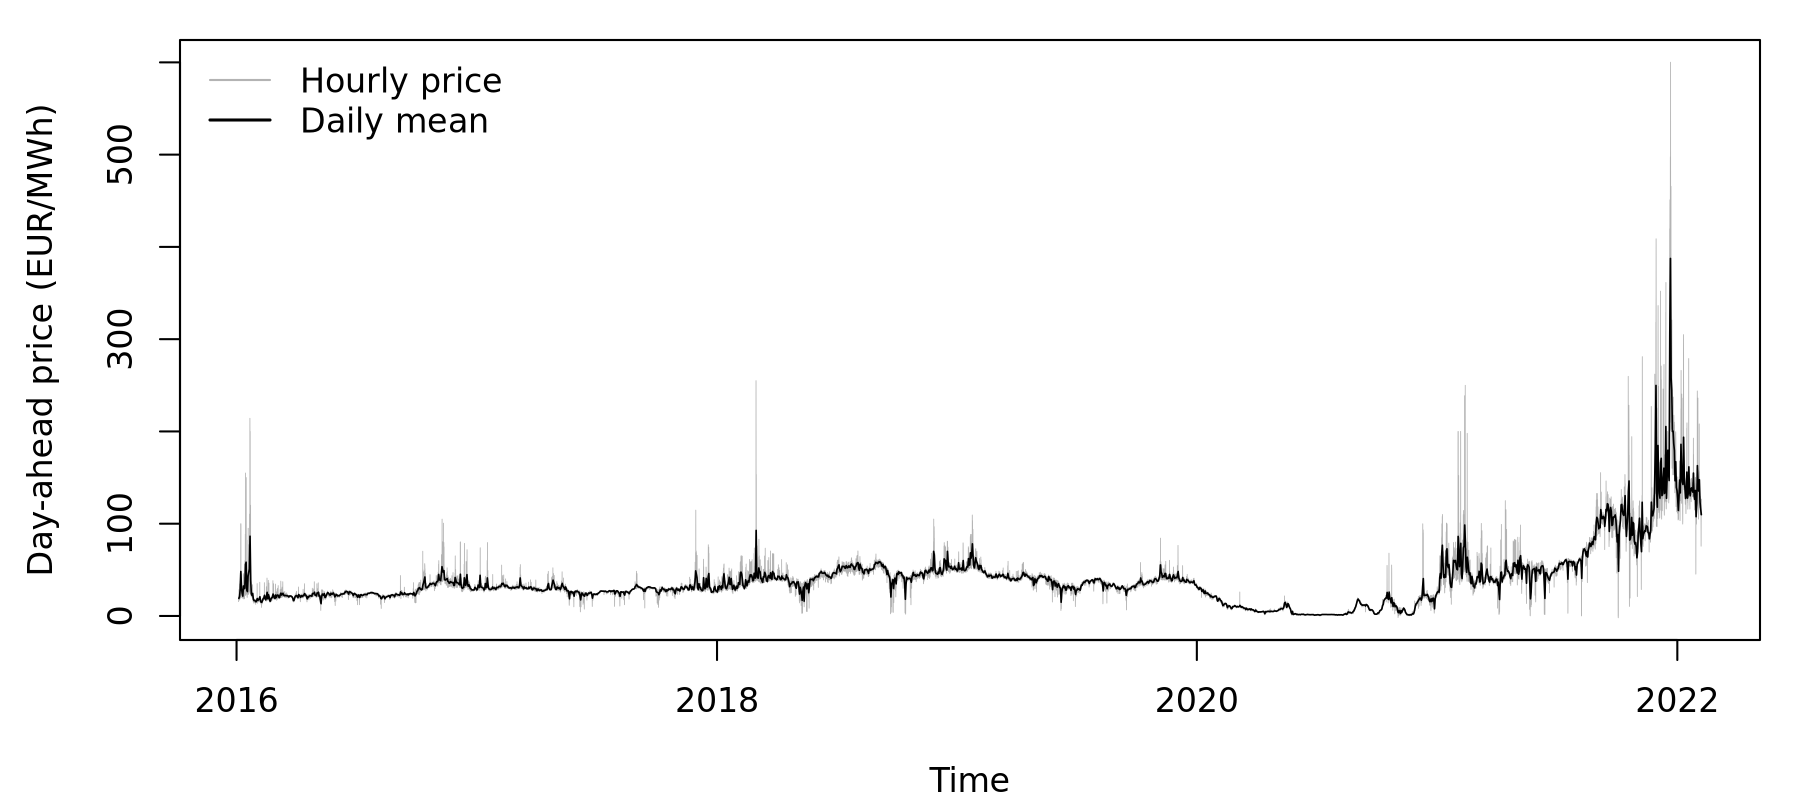
\includegraphics[width=0.85\textwidth]{fig_price_time.png}
\caption{Hourly day-ahead price in NO1 (grey) and daily mean (black).}
\label{fig:time}
\end{figure}

[\textbf{Figure \ref{fig:factors}}] shows the price by hour, month, weekday and year. The price is lowest at night (mean $\hourMinMean$ \eur{} at hour $\hourMinAt$), has a morning peak (mean $\hourMaxMean$ \eur{} at hour $\hourMaxAt$) and a smaller evening peak. The monthly mean is lowest in \monthMinAt{} ($\monthMinMean$ \eur) and highest in \monthMaxAt{} ($\monthMaxMean$ \eur), and weekends are a bit cheaper. The differences between years are much larger than all the other patterns.

\begin{figure}[!htbp]
\centering
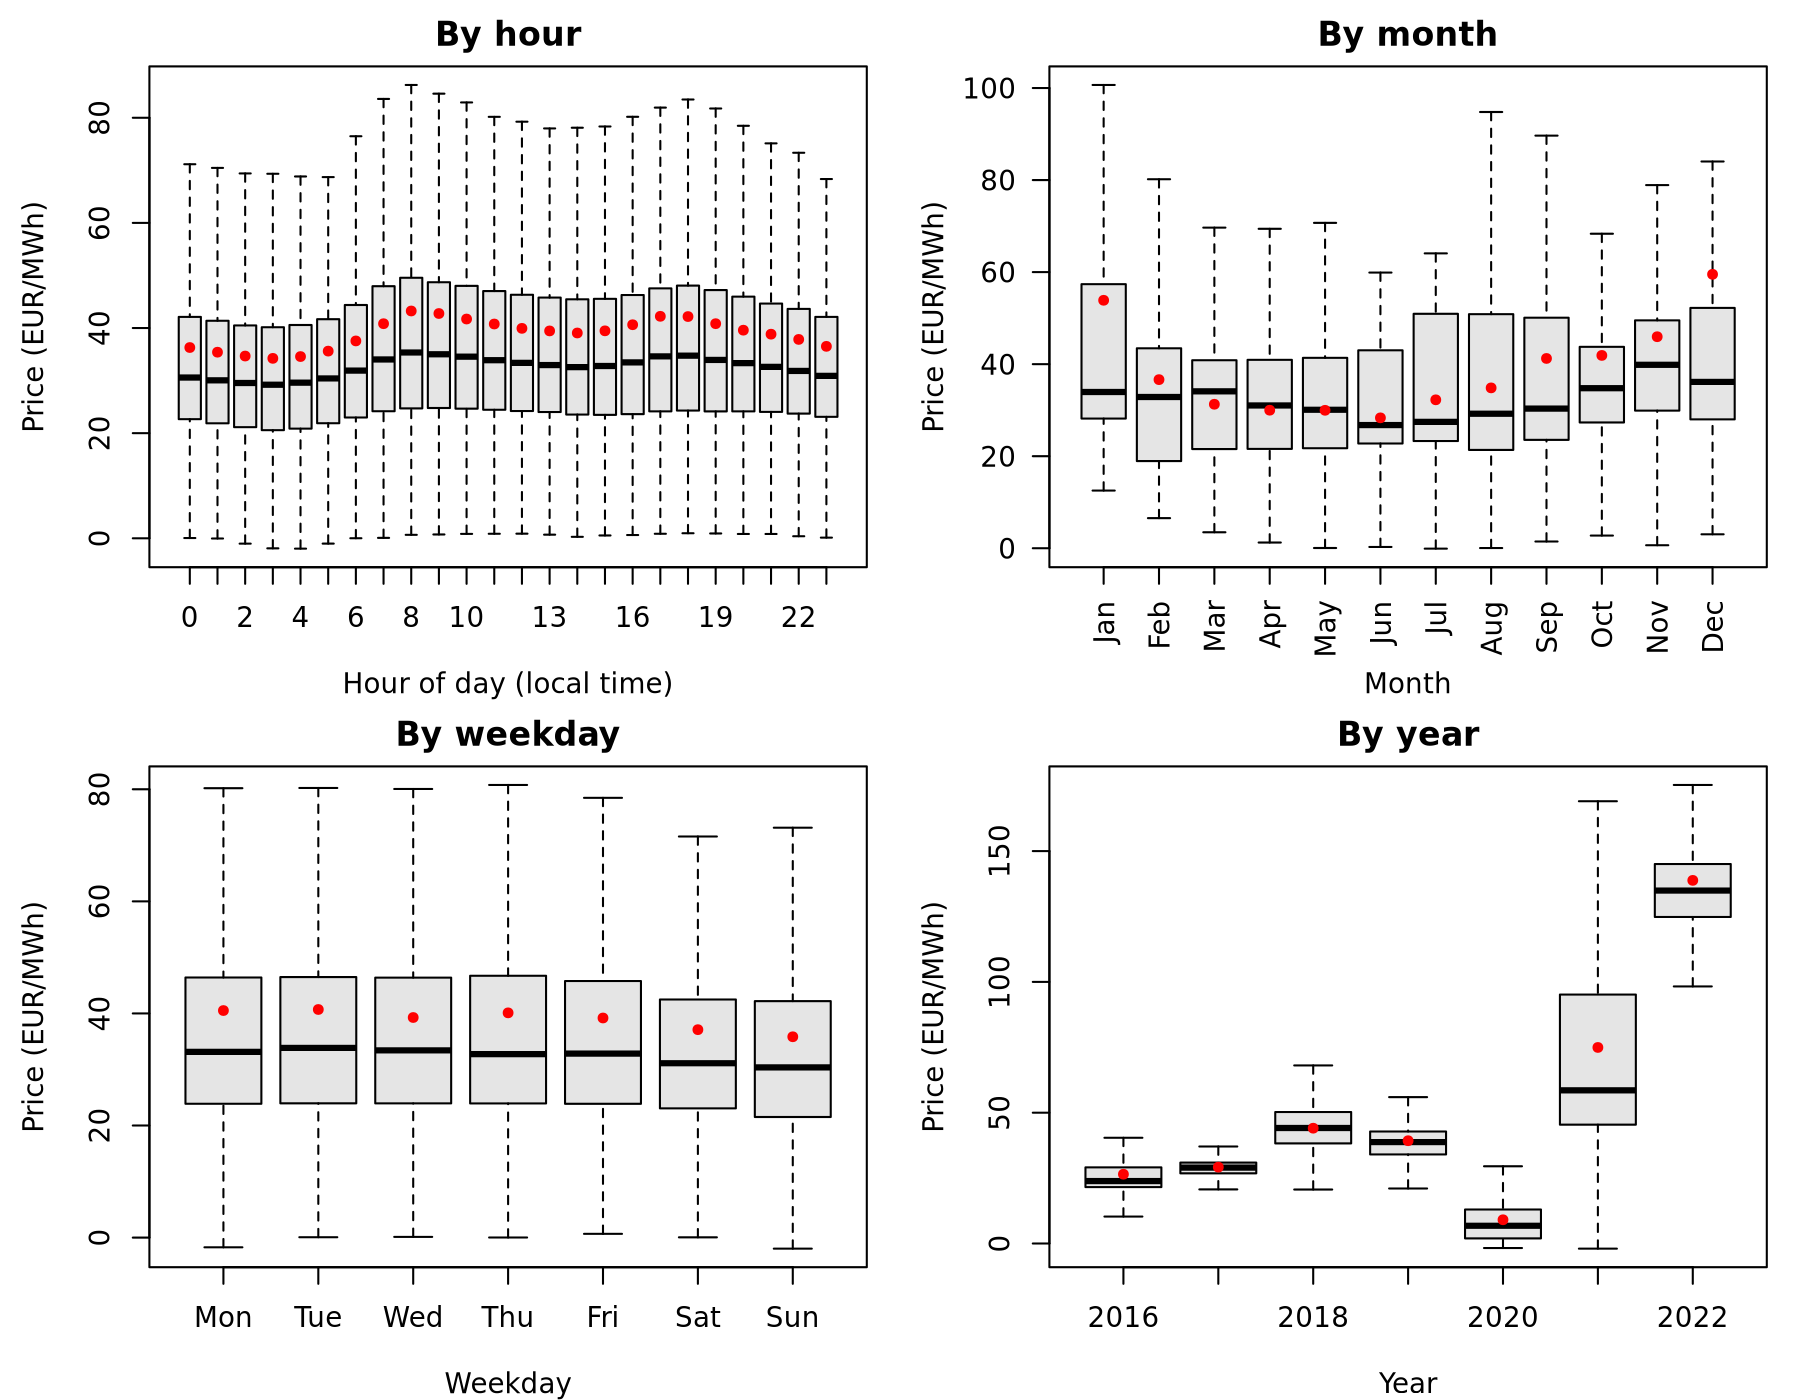
\includegraphics[width=0.75\textwidth]{fig_price_factors.png}
\caption{Price by hour of day, month, weekday and year. Boxes show the quartiles (whiskers without outliers), red points the means.}
\label{fig:factors}
\end{figure}

[\textbf{Figure \ref{fig:scatter}}] shows the price against consumption and reservoir level. The price goes up with consumption, a bit faster at high consumption. Against the reservoir level the pattern is not a straight line: the price is high at low and medium fill levels and drops clearly above about 80\%. The simple correlations are small, $\corPriceCons$ with consumption and only $\corPriceRes$ with reservoir level. One reason is that a correlation mixes all the years, and a fill level of 60\% occurs in both cheap and expensive years. This is why I need a model that holds year and season fixed. Reservoir and consumption have correlation $\corConsRes$, while year (as a number) is almost uncorrelated with both ($\corYearRes$ and $\corYearCons$).

\begin{figure}[!htbp]
\centering
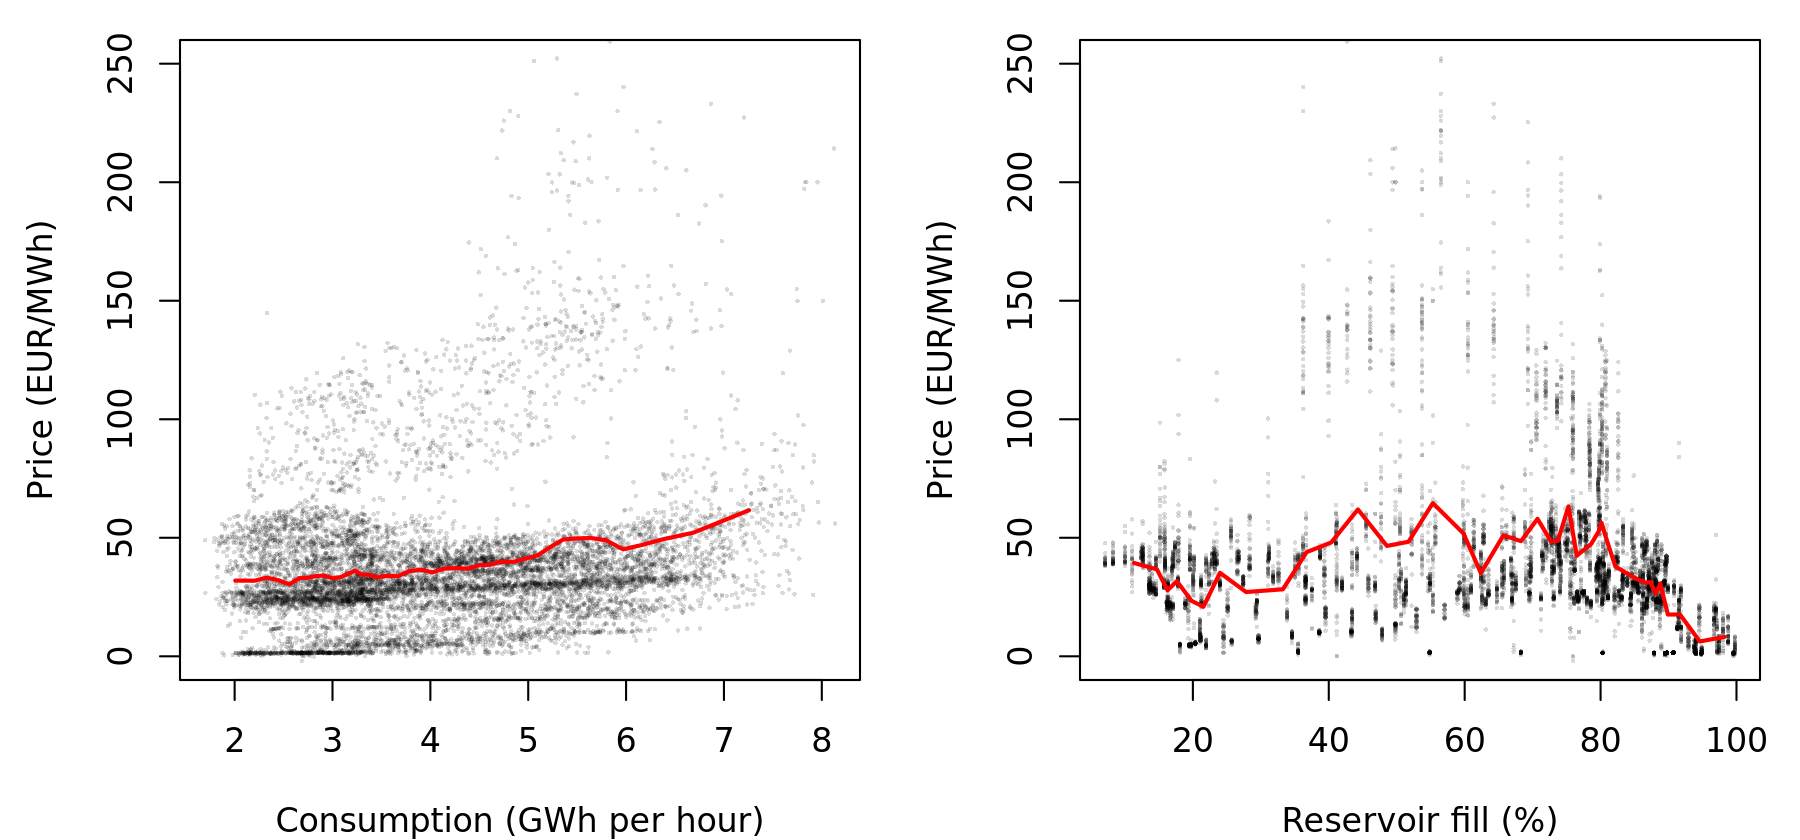
\includegraphics[width=0.85\textwidth]{fig_price_vs_x.png}
\caption{Price against consumption and reservoir fill (random sample of \nScatterSample{} hours, cut at 250 \eur). The red line is the mean price in 40 equally sized groups using all hours.}
\label{fig:scatter}
\end{figure}

%------------------------------------------------------------
\section{Method}\label{sec:method}

\subsection{Why a Gaussian GLM}

A GLM has a response distribution from the exponential family, a linear predictor $\bs{x}_i^T\bs{\beta}$ and a link function with $g(\mu_i) = \bs{x}_i^T\bs{\beta}$, where $\mu_i = E(Y_i)$ \parencite{dobson2008glm}. The price is continuous, so Poisson (counts) and binomial (proportions, yes/no) do not fit. The Gamma distribution and a log transform need a strictly positive response, but there are $\nNonPos$ hours with zero or negative prices, and I do not want to remove them or add an arbitrary constant. The normal distribution allows any real value and belongs to the exponential family (shown in Assignment 2), so a Gaussian GLM is the natural choice. With the identity link, the canonical link for the normal distribution, the model is multiple linear regression and each coefficient is a difference in \eur, which is easy to explain. The model assumes independent, normally distributed errors with constant variance. Hourly prices will probably break some of this, so I check it in Section~\ref{sec:diag}.

\subsection{Model specification}

With the notation from the course the model is
\begin{align*}
y_i = \bs{x}_i^T\bs{\beta} + e_i, \qquad e_i \sim N(0, \sigma^2), \qquad i = 1, \dots, n,
\end{align*}
with identity link, $E(Y_i) = \mu_i = \bs{x}_i^T\bs{\beta}$, where $y_i$ is the price in hour $i$ and
\begin{align*}
\bs{x}_i^T\bs{\beta} = \beta_0
&+ \sum_{h=1}^{23} \beta^{\text{hour}}_h\, I(\text{hour}_i = h)
+ \sum_{m=2}^{12} \beta^{\text{month}}_m\, I(\text{month}_i = m) \\
&+ \sum_{w=2}^{7} \beta^{\text{wday}}_w\, I(\text{weekday}_i = w)
+ \sum_{t=2017}^{2022} \beta^{\text{year}}_t\, I(\text{year}_i = t)
+ \beta_{\text{cons}}\, \text{cons}_i + \beta_{\text{res}}\, \text{res}_i.
\end{align*}
$I(\cdot)$ is 1 if the condition holds and 0 otherwise, $\text{cons}_i$ is consumption in GWh per hour and $\text{res}_i$ the reservoir fill in percent. This gives $p = \nPar$ parameters. The intercept is the price at hour 00 on a Monday in January 2016 with zero consumption and an empty reservoir, which is not realistic, so I do not interpret it. In R:
\begin{displayquote}
\small\raggedright
\texttt{glm(price \textasciitilde{} fhour + fmonth + fwday + fyear + cons + reservoir,}\\
\texttt{\phantom{glm(}family = gaussian(link = "identity"))}
\end{displayquote}
For the Gaussian GLM the maximum likelihood estimates are the least squares estimates $\bs{b} = (\bs{X}^T\bs{X})^{-1}\bs{X}^T\bs{y}$ with $\mathrm{var}(\bs{b}) = (\bs{X}^T\bs{X})^{-1}\sigma^2$ \parencite{dobson2008glm}, and the 95\% confidence intervals are $b_j \pm 1.96\,\mathrm{SE}(b_j)$.

\subsection{Comparing models and collinearity}

To find which predictors matter most I remove one term at a time. For nested normal models the change in deviance gives the $F$-test
\begin{align*}
F = \frac{(D_0 - D_1)/(p - q)}{D_1/(n - p)},
\end{align*}
where $D_0$ and $D_1$ are the deviances of the smaller and larger model with $q$ and $p$ parameters \parencite{dobson2008glm}. As in Assignment 1, I also use $\text{AIC} = -2l + 2k$ and $\text{BIC} = -2l + k\log(n)$, and the loss in $R^2 = 1 - D/D_{\text{null}}$. With $n = \nClean$ almost any effect will be significant, even when it is too small to matter, so I focus on effect sizes and on how much each term adds to the fit.

In Assignment 2 we saw that when two predictors have correlation $r$, the variance of each slope is multiplied by $1/(1-r^2)$. With many predictors this becomes the variance inflation factor $\text{VIF}_j = 1/(1 - R_j^2)$, where $R_j^2$ is the $R^2$ from regressing predictor $j$ on the others. For factors I use the generalized VIF from the \texttt{car} package \parencite{car}, where $\text{GVIF}^{1/(2\,\text{df})}$ is comparable to $\sqrt{\text{VIF}}$, the inflation of the standard error.

\subsection{Autocorrelation}

The hours come one after the other, so the error in one hour is probably close to the error in the next. I check this with the ACF and PACF of the residuals and the Durbin-Watson statistic
\begin{align*}
DW = \frac{\sum_{i=2}^{n}(e_i - e_{i-1})^2}{\sum_{i=1}^{n}e_i^2} \approx 2(1 - \hat\rho_1),
\end{align*}
which is close to 2 without autocorrelation and close to 0 when it is strong \parencite{lmtest}. The residuals are taken in time order, skipping the removed hours ($\pctLagOneIsHour$\% of consecutive rows are exactly one hour apart). Positive autocorrelation makes the usual standard errors too small, so as a short robustness check I compute HAC (Newey-West) standard errors with the \texttt{sandwich} package \parencite{sandwich}, with 168 lags (one week). The estimates stay the same, only the standard errors change.

\subsection{GAM}

The GLM assumes that the price changes by the same amount for every extra GWh and every extra percentage point of fill. If the plots or residuals show curves, a GAM can replace the straight lines with smooth functions,
\begin{align*}
y_i = \bs{x}_i^{*T}\bs{\beta} + f_1(\text{cons}_i) + f_2(\text{res}_i) + e_i, \qquad e_i \sim N(0, \sigma^2),
\end{align*}
where $\bs{x}_i^{*T}\bs{\beta}$ has the same four factors and $f_1, f_2$ are penalized regression splines. I fitted it with \texttt{mgcv::gam} with the default basis (at most $\kMax$ effective degrees of freedom per smooth) and REML \parencite{mgcvREML, mgcvBook}, and compare it with the GLM by AIC, BIC and an approximate $F$-test.

%------------------------------------------------------------
\section{Results}\label{sec:results}

\subsection{The fitted GLM and the key coefficients}

The full model has $R^2 = \rTwo$, so it explains about $\rTwoPct$\% of the variation in the hourly price, and the residual standard error is $\hat\sigma = \rse$ \eur{} on $\dfRes$ degrees of freedom. Selected coefficients are given in [\textbf{Table \ref{tab:coef}}] (all are in \texttt{tables/glm\_all\_coefficients.csv}), and the hour and month effects are plotted in [\textbf{Figure \ref{fig:effects}}].

\begin{table}[!htbp]
\centering
\caption{Selected coefficients of the Gaussian GLM (\eur). Standard errors and 95\% intervals assume independent errors, which is not true here (Section~\ref{sec:diag}).}
\label{tab:coef}
\small
\begin{tabular}{lrrrr}
\toprule
Term & Estimate & SE & 95\% CI & $p$-value \\
\midrule
(Intercept) & 52.27 & 1.27 & [49.78, 54.77] & \ensuremath{<0.001} \\
Hour 03 (vs 00) & \ensuremath{-}2.04 & 0.59 & [\ensuremath{-}3.19, \ensuremath{-}0.88] & \ensuremath{<0.001} \\
Hour 08 (vs 00) & 5.25 & 0.59 & [4.09, 6.42] & \ensuremath{<0.001} \\
Hour 17 (vs 00) & 4.37 & 0.59 & [3.21, 5.53] & \ensuremath{<0.001} \\
April (vs January) & \ensuremath{-}31.99 & 0.69 & [\ensuremath{-}33.35, \ensuremath{-}30.64] & \ensuremath{<0.001} \\
July (vs January) & 18.65 & 0.75 & [17.17, 20.12] & \ensuremath{<0.001} \\
December (vs January) & 33.41 & 0.45 & [32.53, 34.28] & \ensuremath{<0.001} \\
Saturday (vs Monday) & \ensuremath{-}3.03 & 0.32 & [\ensuremath{-}3.65, \ensuremath{-}2.41] & \ensuremath{<0.001} \\
Sunday (vs Monday) & \ensuremath{-}4.20 & 0.32 & [\ensuremath{-}4.83, \ensuremath{-}3.57] & \ensuremath{<0.001} \\
2018 (vs 2016) & 18.11 & 0.29 & [17.53, 18.69] & \ensuremath{<0.001} \\
2020 (vs 2016) & \ensuremath{-}9.87 & 0.31 & [\ensuremath{-}10.47, \ensuremath{-}9.27] & \ensuremath{<0.001} \\
2021 (vs 2016) & 48.97 & 0.29 & [48.41, 49.54] & \ensuremath{<0.001} \\
2022 (vs 2016) & 108.94 & 0.72 & [107.53, 110.35] & \ensuremath{<0.001} \\
Consumption (per GWh/h) & 2.08 & 0.17 & [1.74, 2.42] & \ensuremath{<0.001} \\
Reservoir (per \%-point) & \ensuremath{-}0.71 & 0.01 & [\ensuremath{-}0.73, \ensuremath{-}0.69] & \ensuremath{<0.001} \\
\bottomrule
\end{tabular}

\end{table}

\begin{figure}[!htbp]
\centering
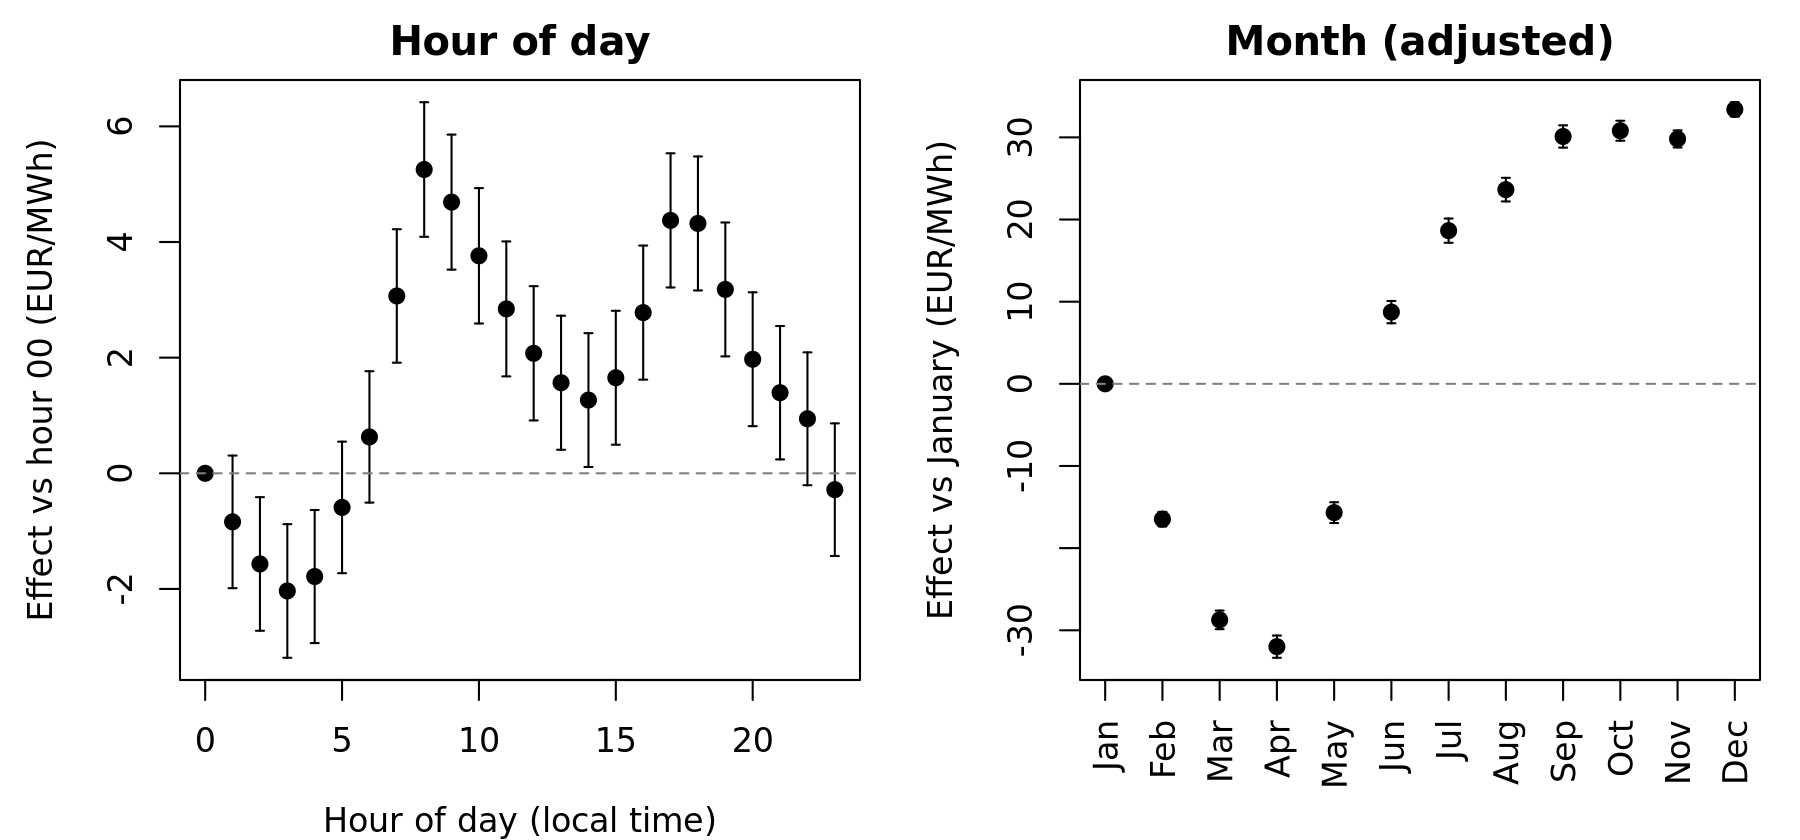
\includegraphics[width=0.85\textwidth]{fig_effects.png}
\caption{Estimated hour effects (vs hour 00) and month effects (vs January) with 95\% intervals, holding the other predictors fixed.}
\label{fig:effects}
\end{figure}

Each coefficient is interpreted holding the other predictors fixed.

\textbf{Hour of day.} Hour $\hNight$ is the cheapest, $\bHourNight$ \eur{} compared with midnight. The morning peak at hour $\hMorning$ is $\bHourMorning$ \eur{} above midnight (95\% CI $[\ciLHourMorning, \ciUHourMorning]$) and the evening peak at hour $\hEvening$ is $\bHourEvening$ \eur{} above. From the cheapest night hour to the morning peak the price rises by about $\peakDiff$ \eur{}, on top of what the hourly consumption already explains.

\textbf{Month.} The month effects do not look like the raw monthly means in [\textbf{Figure \ref{fig:factors}}]. July is $\bJul$ \eur{} above January in the model, even though July has one of the lowest raw means. The model compares months with the same consumption and reservoir level. July normally has low consumption and a filling reservoir, which both lower the price, so a July hour with the same consumption and fill level as a January hour is more expensive. The month effects are what is left of the season after consumption and reservoir level. I come back to this under collinearity.

\textbf{Weekday.} Saturday is $\bSat$ \eur{} and Sunday $\bSun$ \eur{} compared with Monday.

\textbf{Year.} The year effects are by far the largest. Compared with 2016 the price was $\bYeighteen$ \eur{} higher in 2018, $\bYtwenty$ \eur{} lower in 2020, $\bYtwentyone$ \eur{} higher in 2021 and $\bYtwentytwo$ \eur{} higher in early 2022. These are after adjusting for consumption and reservoir level, so the jump in 2021 and 2022 must come from things outside the model, such as fuel and carbon prices in Europe.

\textbf{Consumption.} One extra GWh per hour of consumption is linked with a price $\bCons$ \eur{} higher (95\% CI $[\ciLCons, \ciUCons]$). One standard deviation of consumption ($\sdConsGWh$ GWh/h) corresponds to only $\bConsSD$ \eur.

\textbf{Reservoir level.} One percentage point more water is linked with a price $\bRes$ \eur{} lower, so 10 percentage points give $\bResTen$ \eur{} (95\% CI $[\ciLResTen, \ciUResTen]$), and one standard deviation ($\sdResPct$ points) gives $\bResSD$ \eur. More stored water means a cheaper price, as expected.

\subsection{Which predictors matter most}

[\textbf{Table \ref{tab:drop1}}] shows what happens when each term is removed. All $F$-tests have $p < 0.001$, even the smallest ($F = \minF$ for hour), which is expected with this $n$. The changes in AIC, BIC and $R^2$ are more useful.

\begin{table}[!htbp]
\centering
\caption{Drop-one comparison. Each row removes one term from the full model. $\Delta$AIC and $\Delta$BIC are the increase, $\Delta R^2$ the loss in explained variation.}
\label{tab:drop1}
\footnotesize
\setlength{\tabcolsep}{4pt}
\begin{tabular}{lrrrrrr}
\toprule
Term removed & df & Deviance increase ($10^6$) & $F$ & $\Delta$AIC & $\Delta$BIC & $\Delta R^2$ (\%-points) \\
\midrule
Hour & 23 & 0.15 & 18.1 & 370 & 167 & 0.27 \\
Month & 11 & 3.89 & 1{,}006.4 & 10{,}003 & 9{,}905 & 7.25 \\
Weekday &  6 & 0.11 & 51.3 & 295 & 242 & 0.20 \\
Year &  6 & 23.73 & 11{,}247.2 & 42{,}966 & 42{,}913 & 44.19 \\
Consumption &  1 & 0.05 & 145.6 & 144 & 135 & 0.10 \\
Reservoir &  1 & 1.54 & 4{,}367.6 & 4{,}192 & 4{,}183 & 2.86 \\
\bottomrule
\end{tabular}

\end{table}

Year is clearly the most important term. Removing it reduces $R^2$ by $\dRtwoYear$ percentage points, and the year factor alone gives $R^2 = \rTwoYearOnly$\%. Month comes second ($\dRtwoMonth$ points) and reservoir level third ($\dRtwoReservoir$ points). Hour, weekday and consumption each add less than one point, and consumption has the smallest change in AIC ($\dAICConsumption$). [\textbf{Table \ref{tab:models}}] compares reduced models. The calendar factors alone give $R^2 = \rTwoCal$, and adding reservoir level improves AIC much more than adding consumption.

\begin{table}[!htbp]
\centering
\caption{Model comparison. RSE is the residual standard error in \eur. For the GAM the number of parameters is the total effective degrees of freedom.}
\label{tab:models}
\footnotesize
\begin{tabular}{lrrrrr}
\toprule
Model & Parameters (edf) & AIC & BIC & $R^2$ & RSE \\
\midrule
Calendar factors only & 47 & 446{,}897 & 447{,}321 & 0.637 & 19.58 \\
Factors + consumption & 48 & 446{,}711 & 447{,}144 & 0.639 & 19.54 \\
Factors + reservoir & 48 & 442{,}663 & 443{,}096 & 0.666 & 18.78 \\
Full GLM & 49 & 442{,}519 & 442{,}961 & 0.667 & 18.75 \\
GAM (smooth consumption and reservoir) & 64.8 & 437{,}297 & 437{,}880 & 0.700 & 17.81 \\
\bottomrule
\end{tabular}

\end{table}

So the part of my hypothesis that reservoir level matters more than demand is supported, but both are small compared with year and season. Demand adds little once hour and month are in the model, because most of the variation in consumption already follows the calendar.

\subsection{Collinearity}

The GVIF values are in [\textbf{Table \ref{tab:vif}}], and [\textbf{Table \ref{tab:aux}}] shows how much of consumption and reservoir level the other predictors explain.

\begin{table}[!htbp]
\centering
\begin{minipage}[t]{0.42\textwidth}
\centering
\caption{Generalized VIF for the full GLM.}
\label{tab:vif}
\footnotesize
\begin{tabular}{lrrr}
\toprule
Term & GVIF & df & GVIF$^{1/(2\,\mathrm{df})}$ \\
\midrule
Hour & 1.65 & 23 & 1.01 \\
Month & 79.75 & 11 & 1.22 \\
Weekday & 1.12 &  6 & 1.01 \\
Year & 1.47 &  6 & 1.03 \\
Consumption & 7.76 &  1 & 2.79 \\
Reservoir & 11.67 &  1 & 3.42 \\
\bottomrule
\end{tabular}

\end{minipage}\hfill
\begin{minipage}[t]{0.55\textwidth}
\centering
\caption{$R^2$ (\%) when consumption or reservoir is regressed on other predictors.}
\label{tab:aux}
\footnotesize
\setlength{\tabcolsep}{3pt}
\begin{tabular}{lrrrr}
\toprule
Variable & Month & Year & Hour & All other predictors \\
\midrule
Consumption & 76.4 & 1.6 & 8.4 & 87.1 \\
Reservoir & 89.4 & 2.6 & 0.0 & 91.4 \\
\bottomrule
\end{tabular}

\end{minipage}
\end{table}

Reservoir level has GVIF $\vifReservoir$ and consumption $\vifConsumption$, so their standard errors are inflated by about $\vifadjReservoir$ and $\vifadjConsumption$ times. I expected the main problem to be between year and reservoir level, since dry and wet years differ, but the data does not show this: year explains only $\auxResYear$\% of the reservoir level. The real collinearity is with month, which alone explains $\auxResMonth$\% of the reservoir level and $\auxConsMonth$\% of the consumption. This makes sense, since the reservoirs fill every summer and empty every winter, and consumption is high in winter. Month has a large GVIF ($\vifMonth$), but spread over 11 degrees of freedom it is only $\vifadjMonth$ per degree of freedom.

Just like \texttt{min} and \texttt{max} in Assignment 2, the model has a hard time separating the season from consumption and reservoir level. The month, consumption and reservoir coefficients should be read together, and the odd month effects are a direct result of this. The estimates are still unbiased but less precise than they look.

\subsection{Residual diagnostics}\label{sec:diag}

The diagnostic plots are shown in [\textbf{Figure \ref{fig:diag}}].

\begin{figure}[!htbp]
\centering
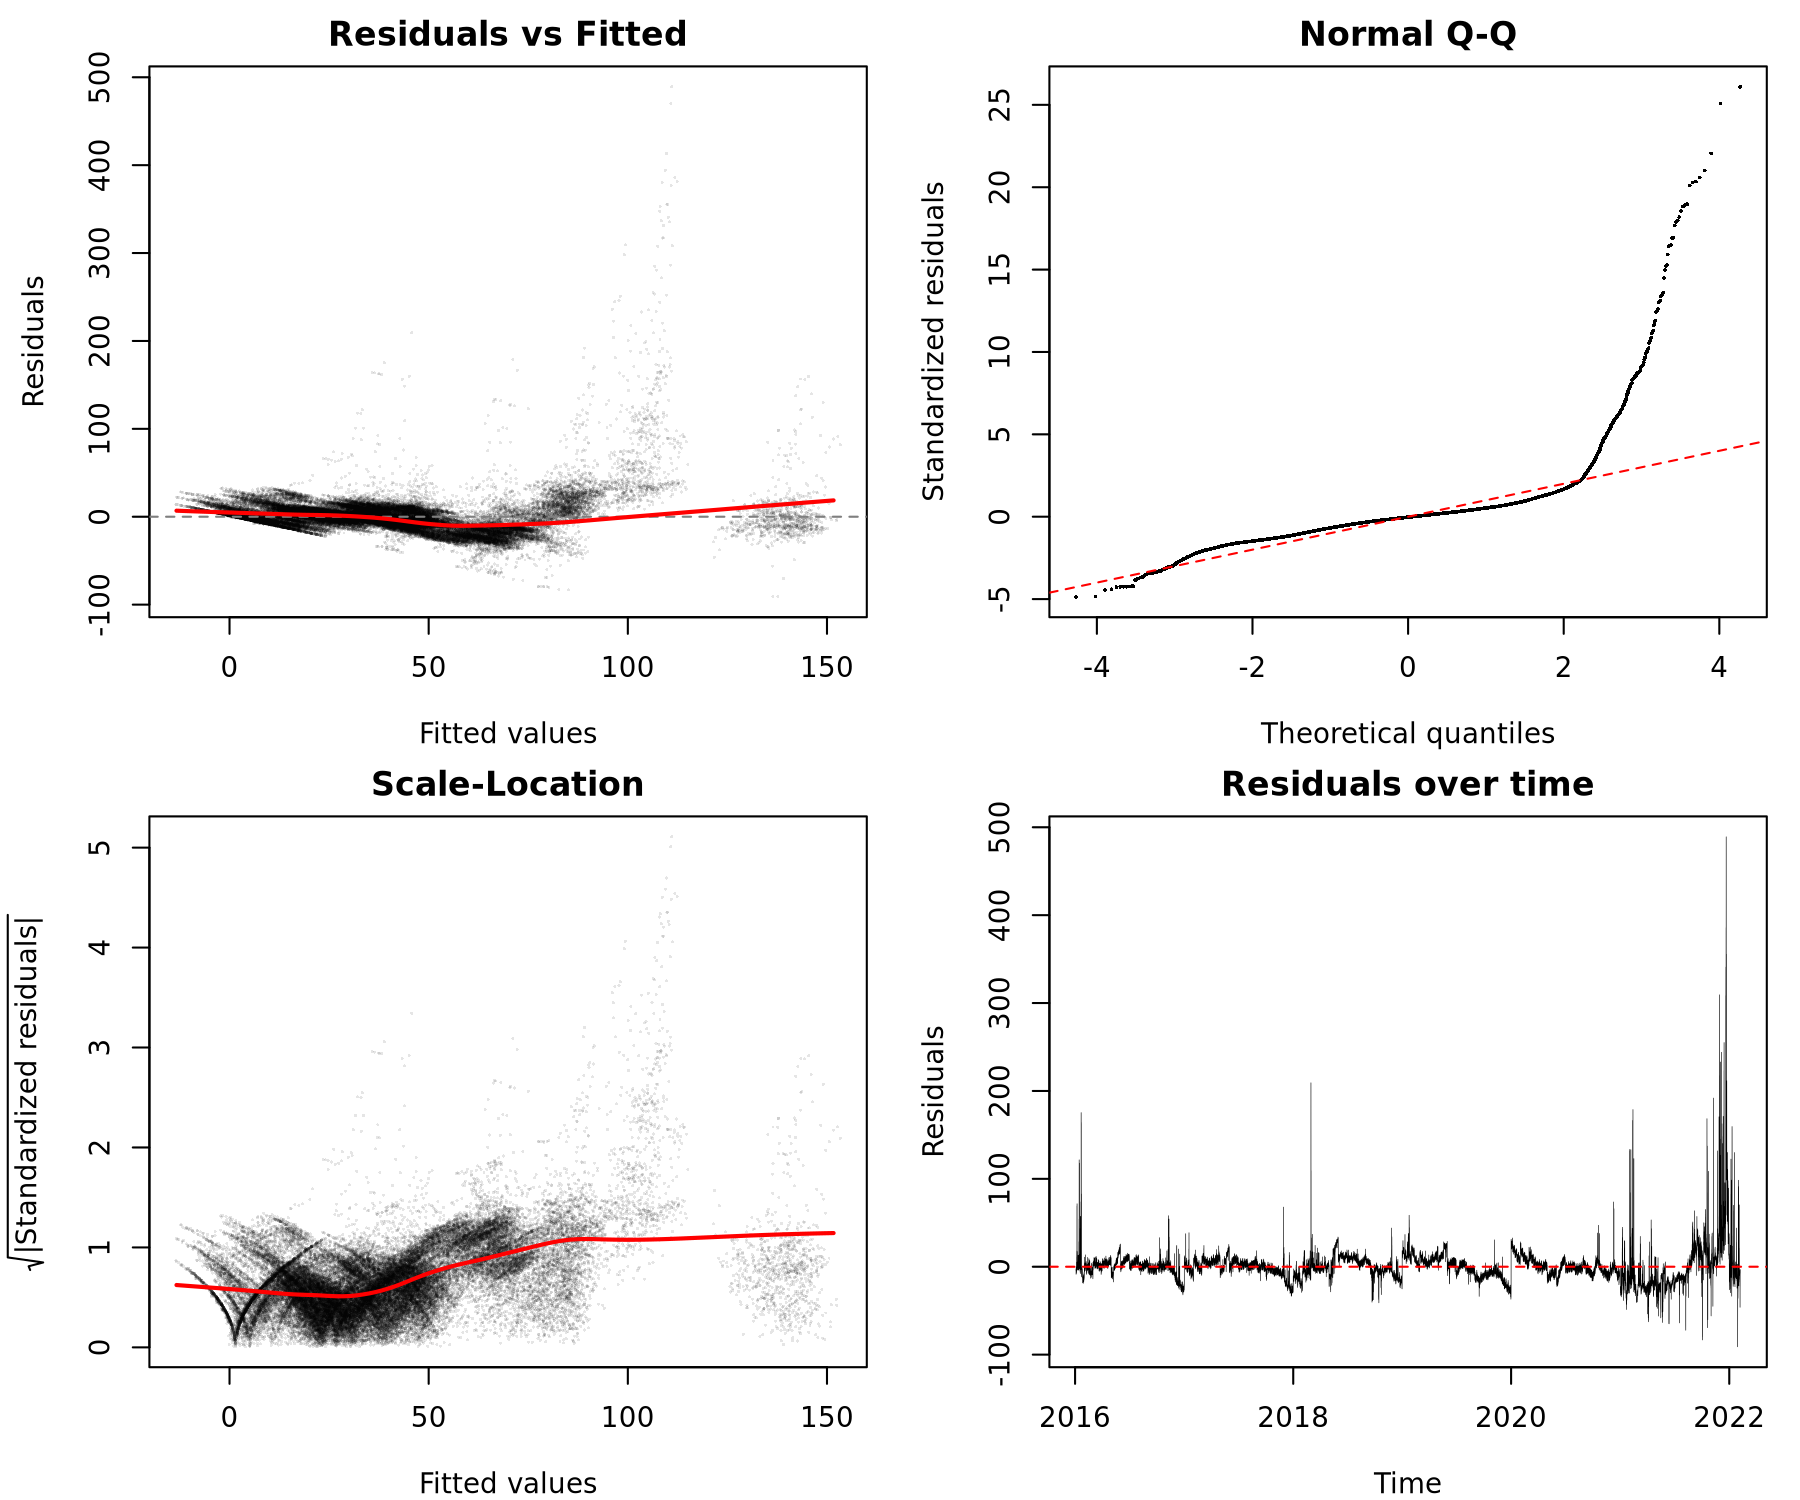
\includegraphics[width=0.78\textwidth]{fig_diagnostics.png}
\caption{Residual diagnostics for the full Gaussian GLM. The red lines in the left plots are lowess smooths.}
\label{fig:diag}
\end{figure}

In the Residuals vs Fitted plot the smooth line bends below zero for fitted values around 50 to 80 \eur{} and there are many large positive residuals at high fitted values, so the model misses some structure. The Scale-Location plot shows that the spread increases with the fitted value, so the variance is not constant. The residual standard deviation is $\resSDYII$ \eur{} in 2017 but $\resSDYVI$ \eur{} in 2021. The Q-Q plot follows the line in the middle but has a very long upper tail: $\pctOutThree$\% of the standardized residuals are beyond $\pm 3$, against about $\pctOutThreeNormal$\% for a normal distribution, and $\pctOutThreeCrisis$\% of these are from September 2021 or later. The residuals over time show long runs above and below zero, which is the sign of autocorrelation. [\textbf{Figure \ref{fig:acf}}] shows the ACF and PACF.

\begin{figure}[!htbp]
\centering
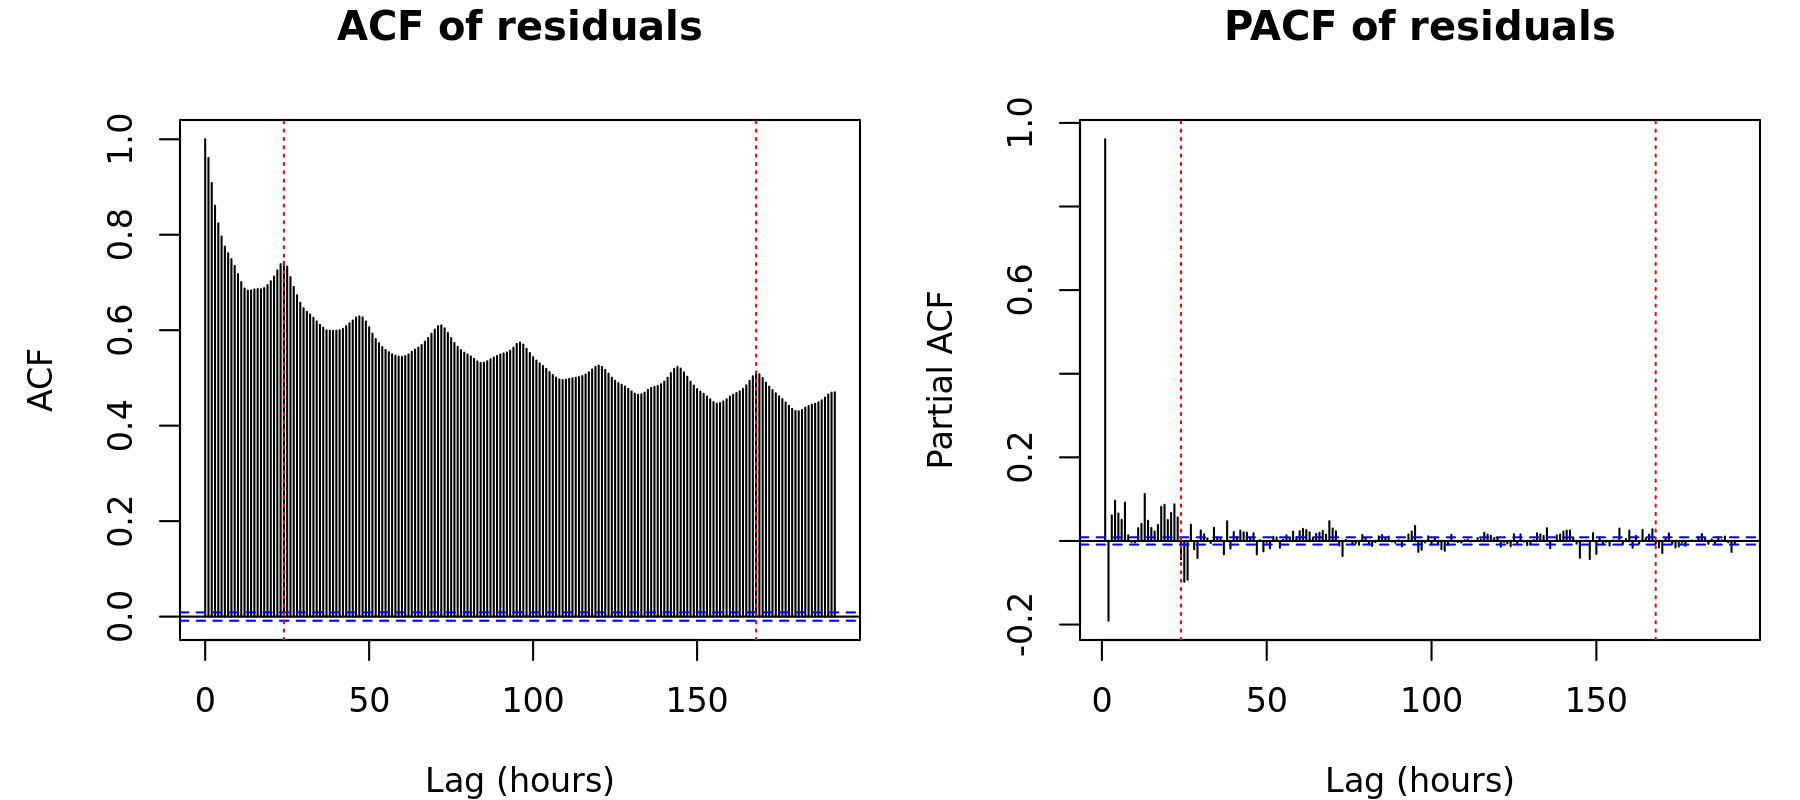
\includegraphics[width=0.85\textwidth]{fig_acf.png}
\caption{ACF and PACF of the GLM residuals in time order, up to 8 days. Red dotted lines mark 24 and 168 hours.}
\label{fig:acf}
\end{figure}

The autocorrelation is $\acfOne$ at lag 1, still $\acfTwentyfour$ at lag 24 and $\acfWeek$ after one week, with small peaks every 24 hours. The PACF is $\pacfOne$ at lag 1 and $\pacfTwo$ at lag 2, and small after that apart from some spikes near lag 24. The Durbin-Watson statistic is $DW = \dw$ ($p$ \dwP), which corresponds to $\hat\rho_1 \approx \dwRho$, far from 2. So the independence assumption is clearly violated. The estimates are still fine on average, but the model treats the $\nClean$ hours as independent information, while one hour tells us almost the same as the next. The standard errors, intervals and $p$-values in [\textbf{Table \ref{tab:coef}}] are therefore too optimistic. [\textbf{Table \ref{tab:hac}}] compares them with HAC standard errors.

\begin{table}[!htbp]
\centering
\caption{Usual and HAC (Newey-West, 168 lags) standard errors. Ratio is SE(HAC)/SE(usual). The estimates are the same.}
\label{tab:hac}
\footnotesize
\setlength{\tabcolsep}{4pt}
\begin{tabular}{lrrrrrr}
\toprule
Term & Estimate & SE (usual) & SE (HAC) & Ratio & $p$ (HAC) & 95\% CI (HAC) \\
\midrule
Hour 08 (vs 00) & 5.25 & 0.59 & 1.35 & 2.3 & \ensuremath{<0.001} & [2.60, 7.91] \\
Hour 17 (vs 00) & 4.37 & 0.59 & 1.30 & 2.2 & \ensuremath{<0.001} & [1.83, 6.92] \\
July (vs January) & 18.65 & 0.75 & 6.76 & 9.0 & 0.006 & [5.39, 31.90] \\
Sunday (vs Monday) & \ensuremath{-}4.20 & 0.32 & 1.02 & 3.2 & \ensuremath{<0.001} & [\ensuremath{-}6.21, \ensuremath{-}2.19] \\
2020 (vs 2016) & \ensuremath{-}9.87 & 0.31 & 2.09 & 6.8 & \ensuremath{<0.001} & [\ensuremath{-}13.98, \ensuremath{-}5.77] \\
2021 (vs 2016) & 48.97 & 0.29 & 4.38 & 15.3 & \ensuremath{<0.001} & [40.38, 57.56] \\
Consumption (per GWh/h) & 2.08 & 0.17 & 1.50 & 8.7 & 0.164 & [\ensuremath{-}0.85, 5.01] \\
Reservoir (per \%-point) & \ensuremath{-}0.71 & 0.01 & 0.15 & 14.1 & \ensuremath{<0.001} & [\ensuremath{-}1.01, \ensuremath{-}0.41] \\
\bottomrule
\end{tabular}

\end{table}

The HAC standard errors are $\hacRatioMin$ to $\hacRatioMax$ times larger. The hour, weekday, year and reservoir effects remain clearly different from zero. For reservoir level the interval for 10 percentage points becomes $[\ciLHacResTen, \ciUHacResTen]$ \eur{} instead of $[\ciLResTen, \ciUResTen]$. The consumption effect does change: its HAC interval is $[\ciLHacCons, \ciUHacCons]$ with $p = \pHacCons$, so taking autocorrelation into account I cannot say that consumption has an effect beyond the calendar factors. Since the autocorrelation is still $\acfWeek$ after a week, even the HAC standard errors are probably somewhat too small.

\subsection{GAM}

[\textbf{Figure \ref{fig:scatter}}] already suggested that reservoir level is not linearly related to the price. To check this inside the model, [\textbf{Figure \ref{fig:residx}}] plots the GLM residuals against the two variables. If the straight line were right, the mean residual would stay near zero.

\begin{figure}[!htbp]
\centering
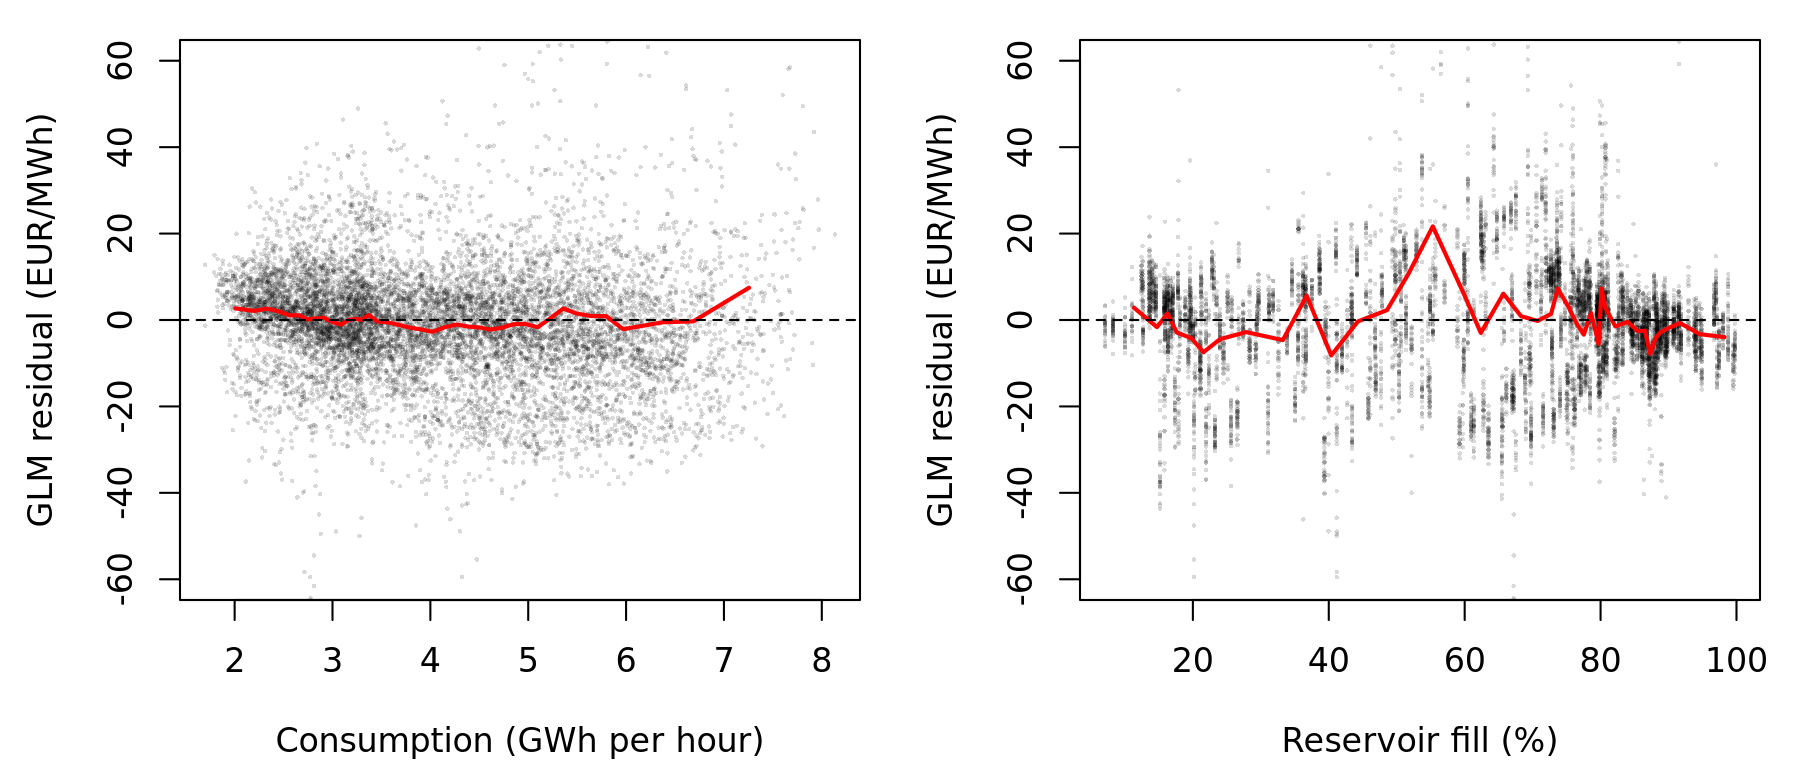
\includegraphics[width=0.85\textwidth]{fig_resid_vs_x.png}
\caption{GLM residuals against consumption and reservoir fill (random sample, cut at $\pm 60$). The red line is the mean residual in 40 equally sized groups using all hours.}
\label{fig:residx}
\end{figure}

In groups of 10\% of the data the mean residual goes from $\binResMin$ to $\binResMax$ \eur{} for reservoir level and from $\binConsMin$ to $\binConsMax$ \eur{} for consumption. Both show a pattern, so I fitted the GAM. The smooth effects are shown in [\textbf{Figure \ref{fig:gam}}] together with the GLM lines.

\begin{figure}[!htbp]
\centering
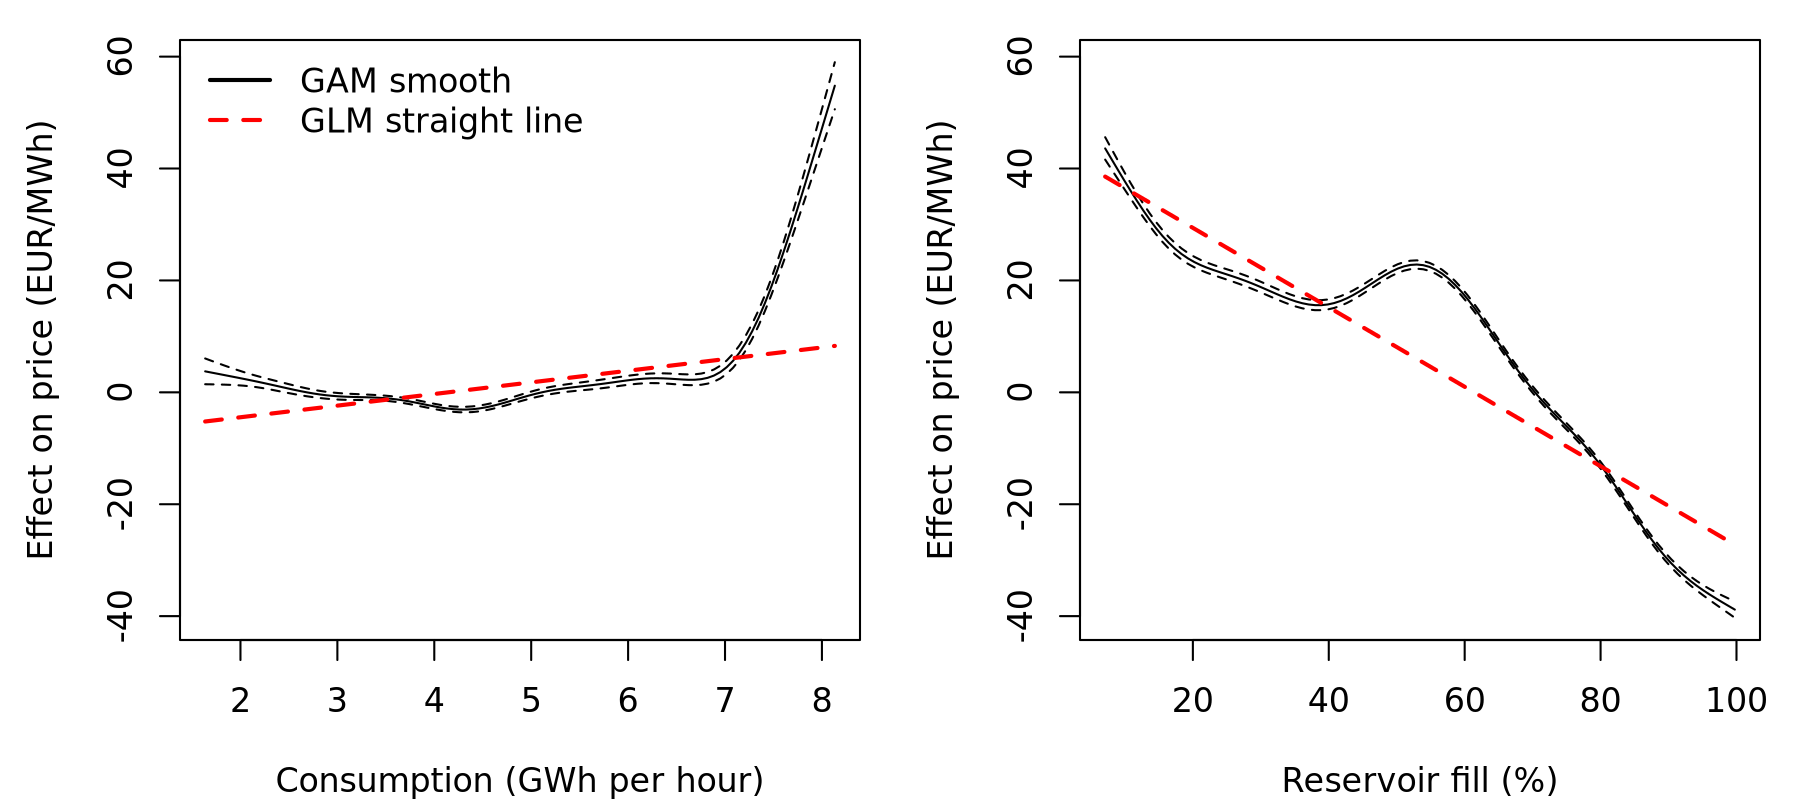
\includegraphics[width=0.85\textwidth]{fig_gam.png}
\caption{Smooth effects from the GAM with 95\% bands (black) and the GLM straight lines (red, dashed). Both are centred, so only shape and differences matter.}
\label{fig:gam}
\end{figure}

The smooths use $\edfCons$ and $\edfRes$ effective degrees of freedom, close to the maximum of $\kMax$. For consumption the curve is almost flat from 2 to 7 GWh/h (a change of $\gamConsTwoToSeven$ \eur) but rises by $\gamConsSevenToEight$ \eur{} from 7 to 8 GWh/h. Only $\nConsAboveSeven$ hours ($\pctConsAboveSeven$\%) are above 7 GWh/h. They are cold winter hours with very high demand, and only $\pctConsAboveSevenCrisis$\% of them are from the crisis period. So consumption hardly matters in normal hours, but the price jumps when demand is extreme.

For reservoir level the price is $\gamResTenToForty$ \eur{} higher at 10\% fill than at 40\%, and falls by $\gamResBumpToNinetyFive$ \eur{} from $\gamResBumpAt$\% to 95\%. The bump between 40\% and $\gamResBumpAt$\% is not a real reservoir effect. For hours with fill between $\binTopLo$ and $\binTopHi$\%, only $\binTopPctDec$\% are from December 2021, but without them the mean GLM residual drops from $\binTopResWithDec$ to $\binTopResNoDec$ \eur. So the bump is mostly the crisis month.

The GAM improves AIC by $\dAICGam$ and BIC by $\dBICGam$ ([\textbf{Table \ref{tab:models}}]), and the $F$-test against the GLM gives $F = \gamF$ on $\gamDf$ extra degrees of freedom ($p$ \gamFp). $R^2$ goes from $\rTwo$ to $\rTwoGam$ and the residual standard error from $\rse$ to $\rseGam$ \eur. The basis check gives a k-index of $\kIndexRes$ for the reservoir smooth, which could suggest a larger basis, but a low k-index is also what we expect with autocorrelated residuals. Autocorrelation also makes the REML smoothing too flexible, so the wiggles should not be over-interpreted.

Is the GAM worth it? It fits clearly better and shows two things the GLM misses: the price jump at extreme consumption, and a reservoir effect that is strongest at low and high fill. But the gain in $R^2$ is moderate, the residual problems remain, and the ranking of the predictors does not change. I therefore use the GLM to interpret the coefficients and the GAM to describe the shape of the two effects.

%------------------------------------------------------------
\section{Discussion}\label{sec:discussion}

The model explains about two thirds of the variation in the hourly price, but most of it comes from the year factor. The year factor tells us \emph{that} the price level was very different in 2020 and 2021, not \emph{why}. It stands in for things outside my data, such as gas and carbon prices in Europe and the export cables. The model is therefore descriptive: it shows how the price varies over the day, week and season and how it is related to the reservoir level, but it does not explain the energy crisis.

My hypothesis was that demand matters and that reservoir level matters even more. The second part is supported. Reservoir level adds much more to the fit than consumption and its effect is robust to autocorrelation. The first part is only weakly supported. Consumption has the expected positive sign, but adds very little once hour and month are known and is not significant with HAC standard errors. The GAM shows why: consumption mainly matters in the most extreme hours.

The most important limitation is the autocorrelation. The usual standard errors are too small, in some cases by more than a factor of 10, and I only used HAC standard errors as a short check. A model that describes the dependence directly, for example with lagged prices, is outside the scope of this course. The variance is also not constant and the residuals have a long upper tail, mostly from the crisis months. Since the price can be zero or negative, a Gamma model or a log transform is not a simple fix.

The collinearity between month, consumption and reservoir level means these coefficients must be read together, while the year and reservoir collinearity I expected was not there. With $\nClean$ hours almost every effect is significant, also weekday effects of one or two \eur{} that hardly matter, which is why I focused on effect sizes, AIC, BIC and $R^2$. Finally, the reservoir level is only measured weekly, $\pctRemoved$\% of the hours were removed, 2022 covers only five weeks, and NO1 is connected to the other Nordic zones, so the price also depends on conditions outside NO1.

%------------------------------------------------------------
\section{Explanation for a non-statistical audience}\label{sec:plain}

I wanted to find out what makes electricity expensive or cheap in the Oslo region, hour by hour. I used about $\nClean$ hours of prices from 2016 to early 2022 and built a model that looks at the time of day, the month, the weekday, the year, how much electricity is used, and how full the hydro reservoirs are.

The biggest difference is between years. Prices were very low in 2020 and then exploded in 2021 and early 2022, and this jump is not explained by how much power was used or how much water was stored. It came from outside factors, such as gas prices in Europe.

Within a year the season matters most, and next is the water in the reservoirs: when the reservoirs are 10 percentage points fuller, the price is on average about $\bResTenAbs$ euro per MWh lower. The time of day has a smaller but clear effect. Electricity is cheapest around \hourMinAt{} at night and most expensive around \hourMaxAt{} in the morning, about $\peakDiff$ euro per MWh more. Weekends are a few euros cheaper. Surprisingly, the amount of electricity used adds little once we know the hour and the month, because usage mostly follows the clock and the calendar. The exception is very cold hours with record demand, when the price jumps.

The model explains about two thirds of the ups and downs in the price. One warning: the price in one hour is very similar to the price in the next, so the data contains less independent information than the number of hours suggests. The main conclusions survive when I correct for this, but the model describes patterns and should not be used to predict exact prices.

%------------------------------------------------------------
\section{Conclusion}

A Gaussian GLM with identity link fits the type of response, since the hourly NO1 price is continuous and can be zero or negative. The model explains $R^2 = \rTwo$ of the variation in $\nClean$ hourly prices. The year is by far the most important predictor, then month and reservoir level. Ten percentage points more water is linked with a price about $\bResTenAbs$ \eur{} lower, while consumption adds very little and is not significant with autocorrelation-robust standard errors. The residuals are strongly autocorrelated (lag-1 autocorrelation $\acfOne$, Durbin-Watson $\dw$), have non-constant variance and a heavy upper tail, so the usual standard errors are far too optimistic. A GAM confirms non-linear effects and improves AIC by $\dAICGam$, but does not change the main conclusions.

\begingroup\sloppy
\printbibliography[heading=bibintoc, title={References}]
\endgroup

\end{document}
